\documentclass[11pt]{article}
\usepackage[margin=1in]{geometry}
\usepackage{tikz}
\usetikzlibrary{positioning,arrows,fit,backgrounds}

\pgfdeclarelayer{background layer}
\pgfsetlayers{background layer,main}
%===========================================================================================
\newcounter{linecounter}
% #1 first line content
\newcommand{\firstline}[1]{
	\setcounter{linecounter}{0}
	\node [anchor=west] (root) {#1}
}

% #1 line tabs
% #2 line content
\newcommand{\nline}[2]{
	\stepcounter{linecounter}
	\node [below=\value{linecounter}*5mm of root.west,anchor=west,xshift=#1*10mm] {#2}
}
%===========================================================================================
%\setlength{\parindent}{0pt}
\begin{document}

test line testasdf asfasdfsfsdfsdfs asdfsd fakjasdfj asdfkjsakfa adsfjkasfasasdf
asfsf asdfsdf asdfsdfflkfasdf adf kadfjadf asdf asdfjkdasdf fasdf.

\noindent
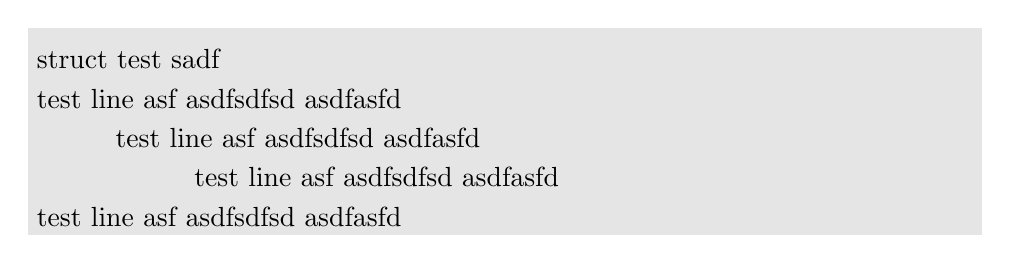
\begin{tikzpicture}
	% On main layer
	\firstline{struct test sadf};
	\nline{0}{test line asf asdfsdfsd asdfasfd};
	\nline{1}{test line asf asdfsdfsd asdfasfd};
	\nline{2}{test line asf asdfsdfsd asdfasfd};
	\nline{0}{test line asf asdfsdfsd asdfasfd};

	% On background layer
	\begin{pgfonlayer}{background layer}
	\fill [gray!20] (current bounding box.south west) rectangle(\textwidth,0.4);
	\end{pgfonlayer}

\end{tikzpicture}

oasdf

\noindent
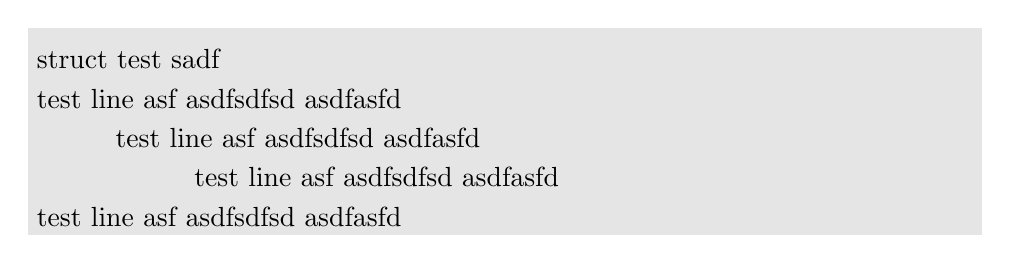
\begin{tikzpicture}
	% On main layer
	\firstline{struct test sadf};
	\nline{0}{test line asf asdfsdfsd asdfasfd};
	\nline{1}{test line asf asdfsdfsd asdfasfd};
	\nline{2}{test line asf asdfsdfsd asdfasfd};
	\nline{0}{test line asf asdfsdfsd asdfasfd};

	% On background layer
	\begin{pgfonlayer}{background layer}
	\fill [gray!20] (current bounding box.south west) rectangle(\textwidth,0.4);
	\end{pgfonlayer}

\end{tikzpicture}
\end{document}
%===========================================================================================
